\documentclass{report}

\usepackage[margin=1in]{geometry}
\usepackage{amsmath,amsthm,amssymb}
\usepackage{enumitem}
\usepackage{graphicx}
\usepackage{caption}

\begin{document}
% ------------------------------------------ %
%                 START HERE                 %
% ------------------------------------------ %
\title{
CS5785 Homework 1\\
	\begin{large}
		Applied Machine Learning
	\end{large}
}
\author{Thomas Matecki}
\maketitle
\section*{Programming Exercises}

\begin{enumerate}
	\item Digit Tokenizer
	\begin{enumerate}[label=(\alph*)]
		\item 
		Training and test data are located in files \textit{train.csv} and \textit{test.csv} respectively. The training data comprises 42000 images and the test data comprises 28000 images.

		\item Figure 1 is one of each digit(0-9) displayed as a 28 by 28 pixel grid.  
		\begin{center}
		\captionof{figure}{}
		\includegraphics[width=12cm]{one_of_each_digit.png}
		\end{center}
		Alternatively, the digit images can be plotted as one dimensional vectors (length = 784).
		\begin{center}
		\captionof{figure}{}
		\includegraphics[width=12cm]{Figure_2.png}
		\end{center}
		\newpage
		\item The distribution of digits within the training data is nearly uniform.
		\begin{center}
		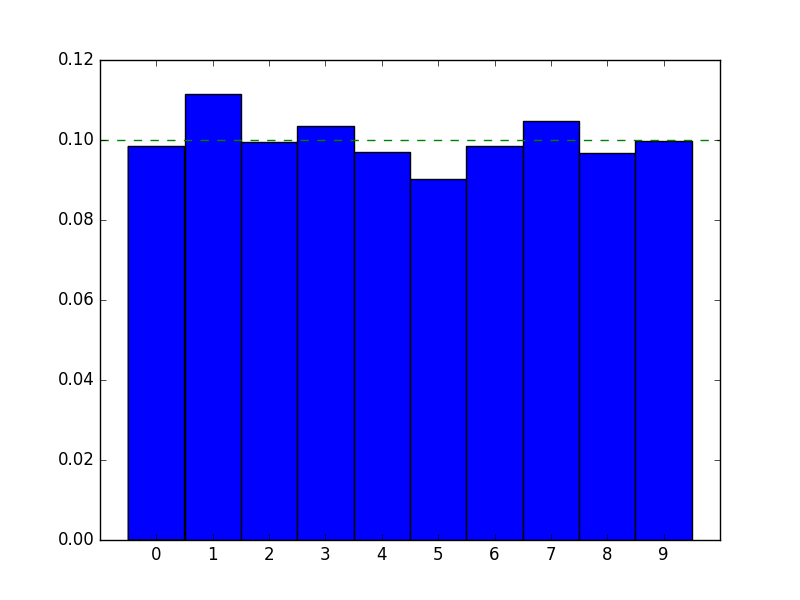
\includegraphics{distrib.png}
		\end{center}	
		\item
	\end{enumerate}
	
	\item The Titanic Disaster
	\begin{enumerate}[label=(\alph*)]
		\item Pro
		\item 
	\end{enumerate}
	
\end{enumerate}

\section*{Written Exercises}
\begin{enumerate}[label=(\alph*)]
	\item Pro
	\item
\end{enumerate}

\end{document}
 